\documentclass[12pt,a4paper]{article}
\usepackage[paper=a4paper, margin=.88in]{geometry}
\usepackage{pdfpages}
\usepackage[utf8]{inputenc}
\usepackage{multicol}
\usepackage{titlesec}
\usepackage{amsmath}
\usepackage{amssymb}
\usepackage{breqn}
\usepackage[english]{babel}
\usepackage[backend=biber,style=numeric]{biblatex}
\usepackage{graphicx,float}
\usepackage[noend]{algorithmic}
\usepackage{multirow}
\usepackage[compact]{titlesec}

\addbibresource{bib.bib}

\titleformat*{\section}{\SMALL\bfseries}
\titleformat*{\subsection}{\SMALL\bfseries}

\begin{document}
\begin{titlepage}

\newcommand{\HRule}{\rule{\linewidth}{0.5mm}} % Defines a new command for the horizontal lines, change thickness here

\center 
 
%----------------------------------------------------------------------------------------
%	HEADING SECTIONS
%----------------------------------------------------------------------------------------

\textsc{\LARGE Vrije Universiteit Amsterdam}\\[1.5cm] 
\textsc{\Large Bachelor Thesis}\\[0.5cm] 

%----------------------------------------------------------------------------------------
%	TITLE SECTION
%----------------------------------------------------------------------------------------

\HRule \\[0.4cm]
{ \huge \bfseries DDO-MCTS: Evaluating O-MCTS with Per-Decision Option Discounting}\\[0.4cm] 
\HRule \\[1.5cm]
 
%----------------------------------------------------------------------------------------
%	AUTHOR SECTION
%----------------------------------------------------------------------------------------

\begin{minipage}{0.4\textwidth}
\begin{flushleft} \large
\emph{Author:}\\
Kevin \textsc{Waller} \\
Vrije Universiteit Amsterdam
\end{flushleft}
\end{minipage}
~
\begin{minipage}{0.4\textwidth}
\begin{flushright} \large
\emph{Supervisor:} \\
Dr. Diederik \textsc{Roijers} \\
Vrije Universiteit Amsterdam
\end{flushright}
\end{minipage}\\[1cm]
~
\begin{minipage}{0.4\textwidth}
\begin{flushleft} \large
\emph{Second Reader:} \\
Dr. Patrick \textsc{Mannion} \\
National University of Ireland Galway
\end{flushleft}
\end{minipage}
~
\begin{minipage}{0.4\textwidth}
\begin{flushright} \large
\emph{Advisor:} \\
Maarten \textsc{de Waard}
\end{flushright}
\end{minipage}\\[2cm]


%----------------------------------------------------------------------------------------
%	DATE SECTION
%----------------------------------------------------------------------------------------

{\large July 2019}\\[2cm] % Date, change the \today to a set date if you want to be precise

%----------------------------------------------------------------------------------------
%	LOGO SECTION
%----------------------------------------------------------------------------------------


\includegraphics[width=4cm]{vu-logo-notext.png}
 
%----------------------------------------------------------------------------------------

\vfill % Fill the rest of the page with whitespace

\end{titlepage}


\begin{abstract}
\textbf{
General Video Game playing is a popular way of benchmarking many artificial intelligence game playing algorithms. One such benchmark is GVG-AI, an annual competition using the VGDL (Video Game Description Language) in which competitors make agents that play against a suite of 2D arcade-style games. The goal is to create an agent that performs well on a variety of games with no game-specific knowledge. Monte Carlo Tree Search (MCTS) is one such popular algorithm that has been able to balance well the problem of exploration and exploitation in reinforcement learning, and since its introduction in 2006 by Coulomb et al \cite{Coulom06mcts} has gained significant mainstream media attention as well for its use in DeepMind's AlphaGo algorithm used to beat the expert Go player Lee Sedol \cite{Silver_2016}. Option Monte Carlo Tree Search (O-MCTS) is a variant of MCTS that uses options instead of reasoning on a primitive single state-action level, and allows the agent to look further into the game, as well as achieve subgoals and strategies \cite{de2016monte}. This paper introduces a culmination of O-MCTS and a more flexible kind of discounting called per-decision option discounting developed by Harutyunyan et al \cite{pmlr-v97-harutyunyan19a}, resulting in Decision Discounting Option Monte Carlo Tree Search, or DDO-MCTS for short. In this paper we show how DDO-MCTS on its own, without tuning, shows little performance benefit. However, in the extended section of this thesis, we show the potential of DDO-MCTS when its discount factors are tuned based on option duration.
}
\end{abstract}

\begin{multicols}{2}
\section{Introduction}
General game playing AI is a type of reinforcement learning problem that deals with algorithms that play a variety of games well, such as pacman, space invaders, and Zelda. Algorithms that generally perform well on games, rather than game-specific algorithms, transfer well to other problems, highlighting the need for such general game playing algorithms. Recent developments in game programming have received wide media attention, for instance when IBM DeepBlue beat the chess world champion, Garry Karsparov, in 1996 \cite{Campbell:2002:DB:512148.512152}, or when DeepMind's AlphaGo beat Lee Sedol in the complex game of Go \cite{Silver_2016}. The General Video Game AI competition is an annual competition that features many arcade style games, and represents the game in the popular Video Game Description language. It has become a popular framework against which to bench such general game playing algorithms. An important aspect of GVG-AI is that no game specific knowledge is used. Competitors do not know beforehand what games will be benchmarked, but can train on another set of games before submission. This means that the algorithms submitted will have to be general, rather than game-specific. GVG-AI and a subset of the games in its suite act as the performance benchmark used in this paper.

Monte Carlo Tree Search, or MCTS, is one such popular general game playing algorithm, which constructs a game tree containing statistics about the game states encountered, and then selects the best actions based off of this game tree \cite{Coulom06mcts}. MCTS collects these game tree statistics by running as many simulations as possible at each time step, where the agent is supposed to select its action at each time step. In GVG-AI, the time to act is 40 milliseconds. Within this amount of time, vanilla MCTS runs as many simulations until termination or some maximum tree depth is reached, updating the game tree as it simulates, after which it selects the action leading to the best next state depending on the game tree statistics. Note how the ability to run simulations indicates that MCTS is also a planning algorithm, as it requires access to the dynamics of the environment.

A problem many game playing algorithms face is being able to look further into the game and make subgoals or strategies that ultimately lead to a victory. Options, as described by  allow for agents to have subpolicies that it can use to get from one state to another with a sequence of actions, rather than reasoning on a single action. Abstracting a game playing AI to work on an option based level therefore allows it to look further into the game tree, as it is not locked to simply looking at single state-action pairs.

In this paper we introduce Decision Discounting Option Monte Carlo Tree Search, or DDO-MCTS, which combines O-MCTS featuring high-level planning using options, with an option dependent discount factor called per-decision option discounting, to allow for unique discounting factors to be used for options. Using GVG-AI as a performance benchmark, DDO-MCTS is compared to a variety of other game playing agents.

Additionally, as an extended part of this thesis, this paper explores a form of hyperparameter tuning in order to provide discount $\gamma$ factors for individual options, based on average sampled duration of the options from simulation, called $\gamma_d$ tuning. 

\section{Background}
\subsection{Markov Decision Processes in Reinforcement Learning}
The Markov Decision Process, or MDP, is a mathematical framework used in reinforcement learning to formulate time sequenced decision making algorithms. In an MDP there is an agent and an environment. At each time step, the agent can take some action, and then the environment responds with some new state and a reward for taking that action.

The formal representation of an MDP is a 4-tuple $ \big \langle S, A, T, R \big \rangle$:
\begin{itemize}
  \itemsep0em 
  \item S is the set of states in the MDP
  \item A is the set of actions available to the agent
  \item $T: S \times A \times S \rightarrow \left[0,1\right]$ is the transition function, which gives a probability of transitioning from some state s to s' with action a
  \item $R: S \times A \times S \rightarrow \mathbb{R}$ is the reward function, which gives a reward for some transition from some state s to s' with action a
\end{itemize}

The goal in reinforcement learning is to find some policy $\pi: A \times S \rightarrow \left[0,1\right]$ which, when followed, maximises the cumulative reward received \cite{sutton1998reinforcement}.  Equation \eqref{eq:rl-goal} formalises this concept using $\gamma$ as a discount factor, where $0 < \gamma \leqslant 1$. Discounting is a way to weight earlier rewards more than future rewards, and limits the horizon to how far the agent can care about future rewards.

\begin{equation}
\underset{\pi}{\max} \mathbb{E}_{\pi} \bigg[\sum_{t}^{\infty} \gamma^t r_{t} | s_{0} = s \bigg]
\label{eq:rl-goal}
\end{equation}

Another way of formulating the problem in reinforcement learning is that of the agent interacting with the environment. The agent can be seen as the decision maker, like the player in zelda, whether this be an actual human player or algorithm. The environment is with which the agent interacts. At each timestep, the agent can take an action, after which the environment responds with a reward and new state. Figure \ref{fig:agent-env} shows the agent-environment interaction diagram. At timestep t, the agent takes some action $A_t$ based on the current reward $R_t$ and state $S_t$, after which, in the next timestep $t+1$, the environment responds with the reward $R_{t+1}$ and the next state $\S_{t+1}$. 

\begin{figure}[H]
    \centering
    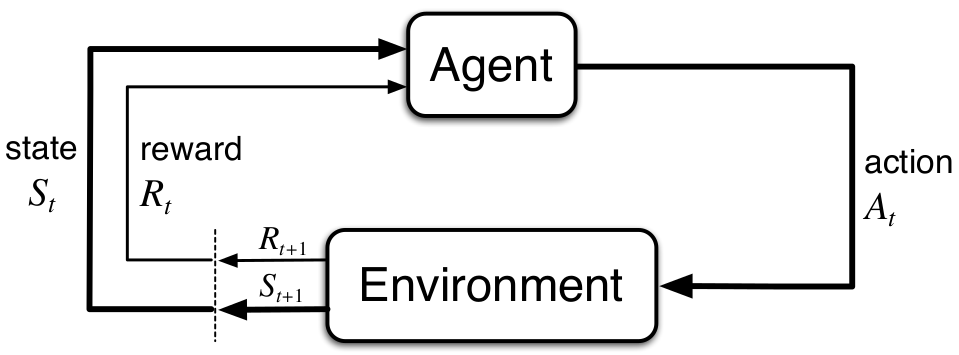
\includegraphics[width=\linewidth]{agent-environment.png}
    \caption{The agent-environment interaction diagram \cite{sutton1998reinforcement}}
\label{fig:agent-env}
\end{figure}

\subsection{Monte Carlo Tree Search \& UCT}
Monte Carlo Tree Search incrementally builds a game tree of statistics by running simulations at each time step, after which it selects the best possible action from the root node. In the next iteration, it does the same, but with the root node as the new current game state of the actual agent. As shown in figure \ref{fig:mcts-phases}, MCTS has four phases; selection, expansion, simulation and backup. In the selection phase, MCTS starts at the root node and uses the tree policy, which propagates down the tree to one of the leaf nodes with a selection strategy called Upper Confidence Bound. At the leaf node, the expansion phase chooses which node is to be added next as the child node of the currently selected node. The simulation phase plays out the rest of the game until termination, at which point the final reward is saved as $\delta$. Usually, the simulation phase picks actions randomly until it reaches some a final state, or until it reaches some maximum search depth, however, heuristics can be used to improve upon a random policy. The final backup phase propagates up the tree from the expanded node, and updates the statistics for all parent nodes that were visited using just $\delta$. This single MCTS iteration is repeated as many times as possible at each time step, after which MCTS chooses the action leading to the best child of the root node. Recall that this single MCTS iteration in GVG-AI happens in 40 milliseconds.

An integral part to MCTS's success is its selection strategy, UCT \cite{Kocsis-Szepesv:2006}.  Balancing exploration of the state space as well as exploitation of the game tree statistics remains a heavily researched and debated topic in reinforcement learning. If the agent chooses actions only based on statistics available, it does not explore the possible other game states in the game that may be much better than what has already been explored. If the agent focuses only on exploration, it will act completely random, and never win the game. UCT, the Upper Confidence Bound for Trees, is a popular formula used for balancing these two factors:

\begin{equation}
	UCT = \frac{w_{s'}}{n_{s'}} + C_p \sqrt{\frac{\ln n_s}{n_{s'}}}
	\label{eq:UCT}
\end{equation}

$w_{s'}$ is the number of wins encountered when passing through this state, whereas $n_{s'}$ is the number of times this nodes has been visited in total. Therefore, the first fraction $\frac{w_{s'}}{n_{s'}}$ is a way of quantifying the quality of a state. This term fully utilises the statistics of the game tree, and thus represents the exploitation term in UCT, since MCTS would not visit any previously unvisited states if selection was based only on this first term in UCT \eqref{eq:UCT}.

$n_s$ is the number of times the parent of s' has been visited, and $n_{s'}$ is the number of times s has been visited. The second term in UCT then represents the exploration term, as nodes that have been visited fewer times than its siblings will have a higher exploration term, increasing the likelihood of the less frequently visited child to be selected. The tune-able parameter $C_{p}$ is the exploration factor, which determines the weight of the exploration term on the UCT value.

During the final backup phase in MCTS, only the last reward, namely $\delta$, is used to update all parent values. The update function varies in MCTS, depending on implementation. A relatively simple update is to add $\delta$ to all parent nodes' values.
\begin{equation}
	v_s \gets v_s + \delta
	\label{eq:backup-vanilla}
\end{equation}
The introduction of a discount factor $\gamma$ changes this vanilla backup function a bit. The backup phase in MCTS works from the bottom up to the top of the tree, whereas regular discounting in equation 1 \eqref{eq:rl-goal} works from the top down the tree. A key difference in MCTS is that only the final reward $\delta$ is used to update all the function values. Since the reward being used to update all states comes from the bottom of the tree, discounting must be done in reverse order, so that the nodes further up the tree are discounted less significantly than those down the tree.
Now the discounting is done as follows, where $s$ is the node to be updated, and $s'$ is the newly created/expanded node:

\begin{equation}
	v_s \gets v_s + \delta\gamma^{d_{s'}-d_{s}}
	\label{eq:backup-discounted}
\end{equation}

MCTS has been used successfully in many game playing algorithms. It gained popularity after two 2006 papers first described and implemented MCTS for the game of Go \cite{Coulom06mcts} \cite{Kocsis-Szepesv:2006}. MCTS proved its ability to deal well with large state spaces when it famously led to the DeepMind team using it to create AlphaGo in 2016 \cite{Silver_2016}. It has also made its way into modern day computer games to act as challenging AI opponents for human players in games like Total War: Rome II \cite{MCTS-total-war}.

\begin{figure}[H]
    \centering
    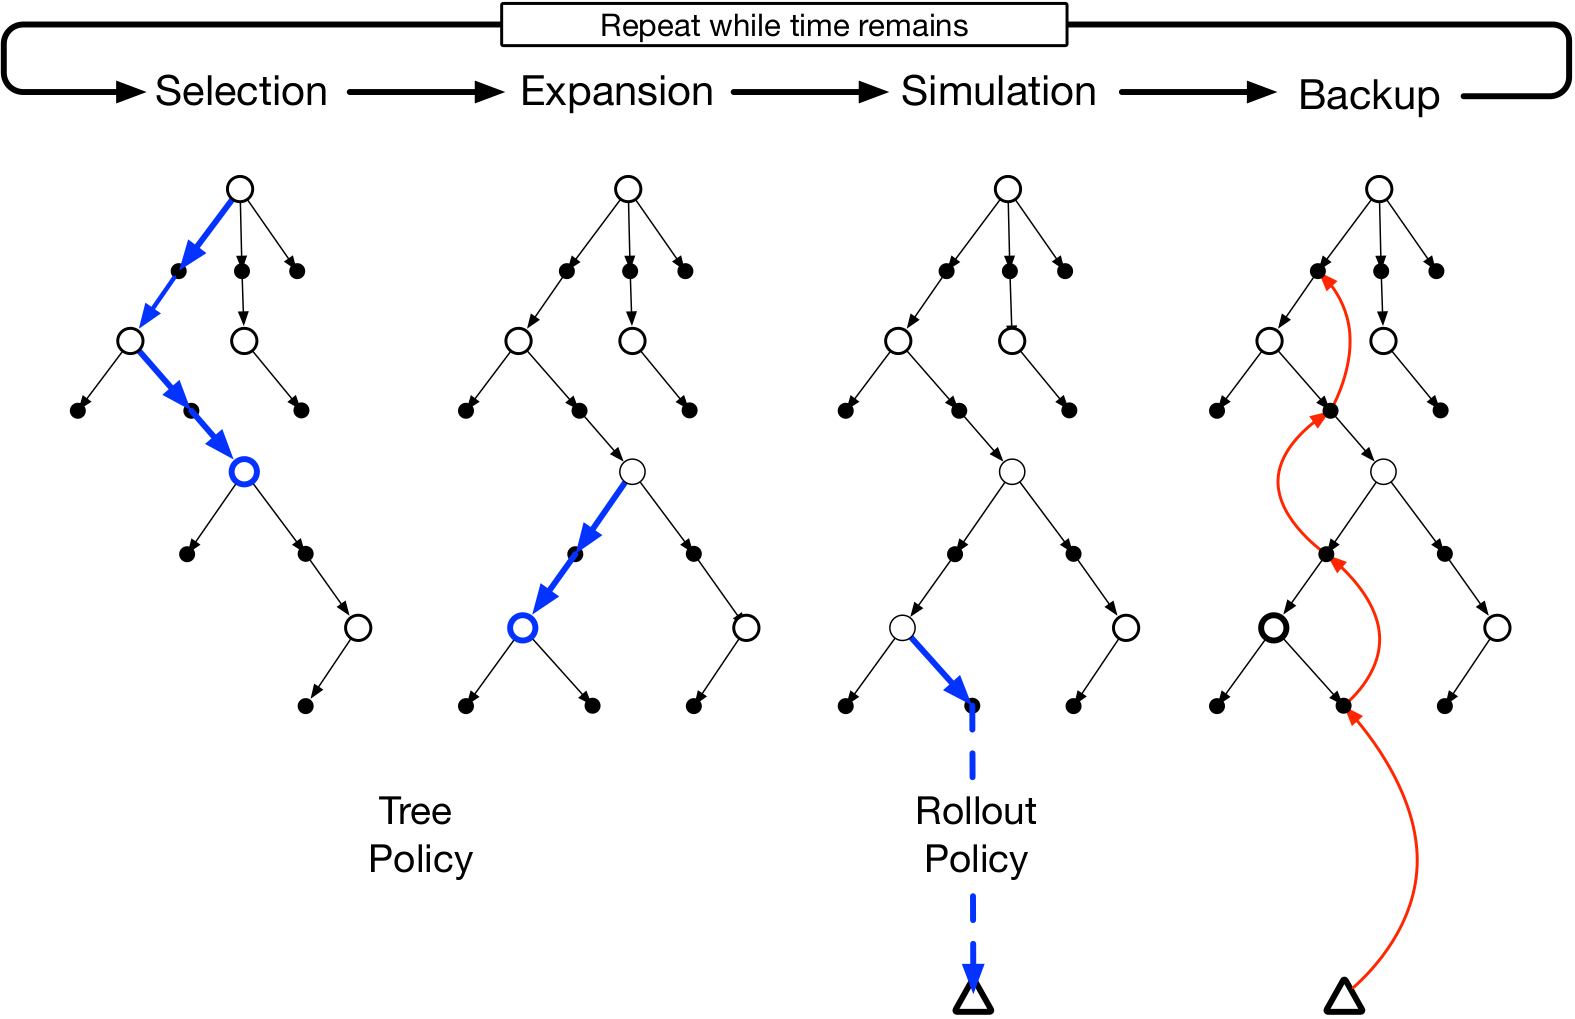
\includegraphics[width=\linewidth]{MCTS-phases.png}
    \caption{The four phases of MCTS. The selection phase uses the tree policy and checks for unexpanded options until a selected node is found. The expansion phase creates a new child node. The simulation phase runs the default policy until termination, upon which delta is received. Lastly, backup updates all visited nodes' statistics in the tree using $\delta$. \cite{sutton1998reinforcement}}
    \label{fig:mcts-phases}
\end{figure}

\subsection{O-MCTS}
Option Monte Carlo Tree Search, or O-MCTS for short, is a variant of MCTS using Options by de Waard et al \cite{de2016monte}.  Options are essentially just a sequence of actions that can bring the agent to a new state that is one or more actions removed from the current state \cite{sutton1999between}.  An agent utilising options can select an option at some time step, instead of just a single action, which represents a sequence of actions. Once some option is selected, the option policy takes over and gets the agent to the new state, after which control goes back to the agent's policy.

Formally, an option o is defined as a 3-tuple $\big \langle I^o, \pi^o, \beta^o \big \rangle$:
\begin{itemize}
    \item $I^o: $ Initiation set, which is the set of states at which option o can start
    \item $\pi^o: A \times S \rightarrow \left[0,1 \right] - $ Option policy, which defines which sequence of actions must be taken to perform option o
    \item $\beta^o: S \rightarrow \left[0, 1\right] - $ Termination condition, which defines when option o has been completed
\end{itemize}

O-MCTS functions exactly the same as regular MCTS, only now the agent can choose to take an option at each time step, rather than a primitive action. This not only allows O-MCTS look further into the game, it also helps it to more easily achieve subgoals. O-MCTS has six predefined options that it can use with VGDL, such as the "GoToPosition" and "WaitAndShoot" options. O-MCTS has shown to perform well on games single player games where the agent and goal have a distinct position, and performs even better in games where there are clear subgoals to be achieved. One game in which O-MCTS performed exceptionally well was zelda, in which one of the levels requires the character to pick up a key in order to unlock a door.

\begin{figure}[H]
    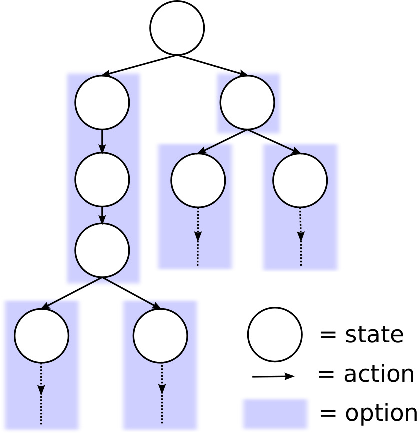
\includegraphics[width=\linewidth]{omcts-eps-converted-to.pdf}
    \caption{Option abstraction in O-MCTS. The blue boxes represent a sequence of nodes that belong to a particular option. \cite{de2016monte}}
\end{figure}

\subsection{Per-Decision Option Discounting}
Per-Decision Option Discounting, as suggested by Harutyunyan et al \cite{pmlr-v97-harutyunyan19a}, is a different kind of discounting for option based reinforcement learning algorithms. Instead of having a single discount factor $\gamma$, there is a set $\Gamma^o = \big\{ \gamma^o_{r}, \gamma^o_{p}, \gamma^o_{d}  \big\}$.
\begin{itemize}
    \item $\gamma^o_{r}$ : The reward discount factor is the same as regular $\gamma$ as shown in equation \eqref{eq:backup-discounted}
    \item $\gamma^o_{p}$ : The transition-step factor is used only within option o, where $\gamma^o_{p} > \gamma^o_{r}$
    \item $\gamma^o_{d}$ : The per-decision state-dependent discount factor is used to discount the entirety of option o
\end{itemize}

A way of formulating the rewards received following some option o using per-decision option discounting $\Gamma$, is done using the probability transition function for option o:
\begin{dmath}
    P^o_{\gamma}\big(s'|s\big) = \gamma_{d}(s')\beta^o\big(s'\big) \bigg(\gamma_{p}p^\pi^o \big(s'|s\big) +  \gamma^2_{p}\sum_{s''}p^\pi^o \big(s''|s\big)(1 - \beta^o  \big(s''\big)\big)\big(p^\pi^o\big(s'|s''\big)+...\big)\bigg)
\end{dmath}

When the agent does not follow an option, $\gamma_{r}$ is used to discount as normal.

Per-decision option discounting allows for time dilation in option based algorithms. By setting $\gamma^o_{p} > \gamma^o_{r}$, the duration of an option matters less, allowing for what Harutyunyan et al refers to as "time dilation". The per-decision discount factor $\gamma^o_{d}$ also allows for the cumulative reward returned from an option to be discounted differently from other options and individual actions. The idea is that, a larger discount factor $\gamma$ when options are being followed, will give the agent some form of foresight.

\section{GVG-AI and VGDL}
The General Video Game AI Competition, sponsored by DeepMind, is the framework used in this paper as a performance benchmark. It contains a large suite of games for different tracks of the GVG-AI competition. The GVG-AI competition has five tracks, of which the  planning and learning tracks are the most popular. Planning algorithms are when agents have access to the environment model, whereas learning algorithms do not. Therefore, learning algorithms learn over many real iterations of games. This make MCTS a planning agent, as it runs many simulations from the current state, then selecting the best action on the statistics collected from these sample games. In this paper specifically, we focus on the single player planning track. This means that board games, such as chess, are not considered.

GVG-AI uses the Video Game Description Language, or VGDL, as first described by Tom Schaul \cite{6633610}. He originally created VGDL in Python, called PyVGDL, for use with pygame, with the aim to have some sort of unified and agreed upon game description standard, making it much easier to write game agents without knowing details about the game, or making it game specific. VGDL allows for a wide variety of video games to be represented in a very simplistic manner, and easily understandable for humans. All games in the GVG-AI single player planning track use Java controllers and the Java-VGDL. This is the track used to benchmark the agents in this paper.

\section{DDO-MCTS}
Decision Discounting Option MCTS is a combination of per-decision option discounting by Harutyunyan et al \cite{pmlr-v97-harutyunyan19a} with Option-MCTS by de Waard et al \cite{de2016monte}. O-MCTS uses regular MCTS discounting as shown in equation \eqref{eq:backup-discounted}. However, having a single discount factor irrelevant of whether or not options are run, limits the agent's ability to consider a bigger payoff for a long-term strategy. In order to implement per-decision option discounting in O-MCTS, options need to have predefined discount factors.

The main modification to O-MCTS is in the backup function. 
% \begin{figure}[H]
%     \caption{OptionBackup for O-MCTS}
%     \begin{algorithmic}
%         \STATE {$\mathbf{function\ OptionBackup}\big(n, \delta, max\_depth\big)$}
%         \WHILE{not $isOptionDone\big(n\big)$}
%             \STATE {$sum \leftarrow sum + \delta{\gamma^{o(n)}_{p}}^{\big(max\_depth - d\big(n\big)\big)}$}
%             \STATE {$n \leftarrow parent\big(n\big)$}
%         \ENDWHILE
%         \STATE {$v\big(n\big) \leftarrow v\big(n\big) + sum{\gamma^{o(n)}_{d}}^{\big(max\_depth - d\big(n\big)\big)}$}
%         \RETURN $n$
%     \end{algorithmic}
%     \bigskip
%     \begin{algorithmic}
%         \STATE {$\mathbf{function\ Backup}\big(n, \delta, max\_depth\big)$}
%         \WHILE{n is not null}
%             \IF{isOptionNode\big(n\big)}
%                 \STATE {$n \leftarrow OptionBackup\big(n, \delta, max\_depth\big)$} \ELSE \STATE{$v\big(n\big) \leftarrow v\big(n\big) + \delta\gamma_{r}^{max\_depth - d\big(n\big)}$}
%             \STATE {$N\big(n\big) \leftarrow N\big(n\big) + 1$}
%             \STATE {$n \leftarrow parent\big(n\big)$}
%         \ENDWHILE
%     \end{algorithmic}
% \end{figure}

\begin{figure}[H]
    \centering
    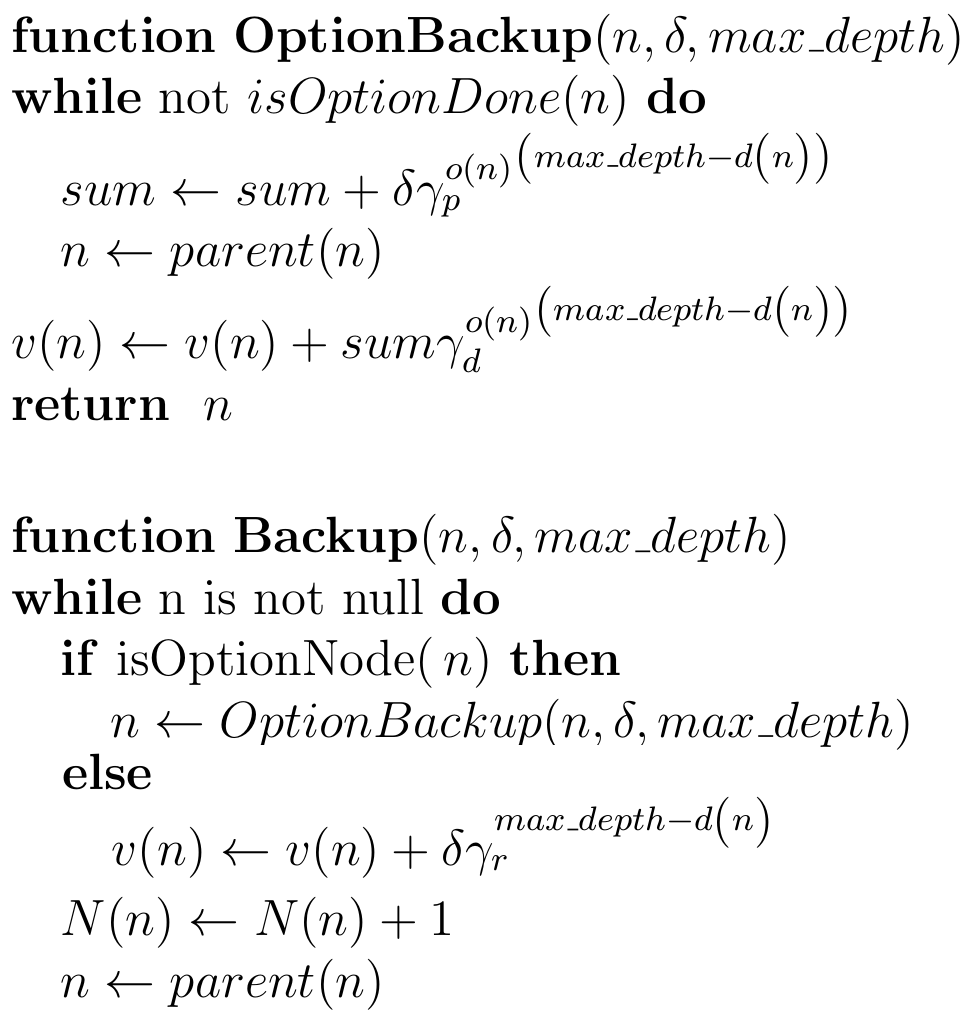
\includegraphics[width=\linewidth]{pseudocode.png}
    \caption{OptionBackup for O-MCTS}
\end{figure}

The function $Backup$ is still the first to be called, with the expanded node being n, $\delta$ being the final reward, and $max\_depth$ being the maximum depth reached during the simulation phase. The while loop checks if an option is in progress or not. If not, it updates the node's statistics using $\gamma_{r}$, where $\gamma_{r} < \gamma_{p}$ for all options.

However, once n is an option node, it calls the $OptionBackup$ function, which accepts the exact same parameters as the $Backup$ function, but instead returns the first node where the option started. As $OptionBackup$ propagates up the tree, it checks if the option is still on going at the current node. If the option is still ongoing, $\gamma_{p}$ is used as the discount factor, and once the entire option has been backpropagated, $\gamma_{d}$ is used for the entire summation and the first node at which the option occurs is updated using this final result. It returns the node back to the $Backup$ function which continues to backpropagate up the tree until the root node is reached.

DDO-MCTS requires $\Gamma$ to be set manually. $\gamma_{r}$ is just a single value, however, a unique $\gamma_{p}$ and $\gamma_{d}$ can be set for each option individually. The default is to keep $\gamma_{p} = \gamma_{r} \approx 0.9$, and $\gamma_{p} \approx 0.95$, to provide a larger horizon for options. Since DDO-MCTS has a total of 6 options to choose from, each having their own unique pair of discount factors $\gamma_{p}$ $\gamma_{d}$, there is a total of 12 discount factors that can be set for options. $\gamma_{r}$ remains a single discount factor.

\section{Results}
\subsection{Experimental Setup}
To benchmark DDO-MCTS's performance, we ran it on a suite of 12 games from GVG-AI, each game being played 100 times in total over 5 difficulty levels, where each level is being played 20 times. Each simulation outputs the winning player, total score as well as number of timesteps to complete the game. To compare performance of DDO-MCTS, benchmarks were ran with two other agents, namely regular MCTS and O-MCTS. MCTS used a non-discounting backup function, the one shown in \eqref{eq:backup-vanilla}, whereas O-MCTS used the discounting in \eqref{eq:backup-discounted} with $\gamma = 0.9$ . DDO-MCTS ran with the default discounting factors, which keeps all discounts the same except for the discounts run within an option $\gamma_{p}$, as this will act as the independent variable in the experiment, where performance measured in win/loss ratio and average score are used as the dependent variable.
The games were run using a desktop computer with a quad core Intel i7-3770k processor and 16GB of DDR3-1600 RAM.

The table below lists the default hyperparameter settings for MCTS, O-MCTS and DDO-MCTS.

\begin{table}[H]
\centering
\begin{tabular}{ll}
\textbf{Parameter Name} & \textbf{Value} \\
Rollout Depth           & 70             \\
Epsilon ($\epsilon$)                 & 1e-6           \\
Exploration Factor ($C_p$)  & $\sqrt{2}$       
\end{tabular}
\caption{Hyperparameter settings for the experiment}
\end{table}

\subsection{Results & Evaluation}
The results are shown in figure \ref{fig:thesis-res}. Some games, like surround and infection, saw little to no improvement, as MCTS, O-MCTS and DDO-MCTS all perform extremely well, shown by their high win ratio. In games like missilecommand, camelRace and chase, although DDO-MCTS still performs significantly better than regular MCTS, little improvement is seen over O-MCTS. Some other games saw performance decrease from MCTS to O-MCTs and DDO-MCTS, suggesting that these games do not benefit much from options, or the options programmed are simply not effective for the game.

The only game in which DDO-MCTS performed significantly better than O-MCTS and MCTS was Zelda. One of the reasons it might have performed better is the fact that the game Zelda relies on a sub-objective to be completed in order to finish the game. In Zelda, the player has to grab a key and open a door, while avoiding/eliminating enemies in the game. DDO-MCTS is likely to perform well in such games, as achieving sub-goals like these is what options and decision discounting is meant for, being able to recognize a larger payoff even though it would take a longer sequence of actions.

The bottom graph in figure \ref{fig:thesis-res} also shows the normalised mean scores for each game. In some cases, like in the games missilecommand, camelRace and seaquest, DDO-MCTS and O-MCTS accumulate a similar score and more than MCTS. However, note how MCTS does have a higher win/loss ratio than DDO-MCTS and O-MCTS in seaquest. In pacman and roguelike, MCTS is seen to perform better than DDO-MCTS and O-MCTS even though the win/loss ratio is the same. Both pacman and roguelike are rather complex games in comparison to some of the other games tested. DDO-MCTS and O-MCTS consistently encountered timeouts where the simulation phase would take too long and cause the GVG-AI controller to select a NULL action. It is possible that this is due to the options that DDO-MCTS and O-MCTS utilise, since options obviously take more timesteps to perform than a primitive action. This highlights a particular weakness for options in MCTS, especially when the time is as restricted as 40 milliseconds as in GVG-AI.

Gradual performance gain can be observed from MCTS to O-MCTS to DDO-MCTS in the games zelda and eggomania. Especially in eggomania, a game in which a chicken throws eggs down which the avatar tries to catch, shows that more reward directly correlates to a higher win/loss ratio, and therefore, better performance. Even though option based methods clearly show improvement over regular MCTS, DDO-MCTS does not seem to accumulate that much more reward on average than O-MCTS, and in some games accumulates fewer average rewards.

From these results, we cannot conclude that DDO-MCTS really does perform better than O-MCTS. However, it is possible that, since the discount factors were not tuned for this experiment, that some form of tuning will provide better results. Per-decision option discounting provides the flexibility to tune these parameters. Performance benefits with tuning are almost certain, but the question is whether or not the payoff for tuning is worth it and whether or not a particular setting will generalise well against many games, or if it will have to be tuned on a game by game basis. This is the topic explored in the thesis extension in section 8, with a process called $\gamma_d$ tuning.

\begin{figure*}
    \centering
    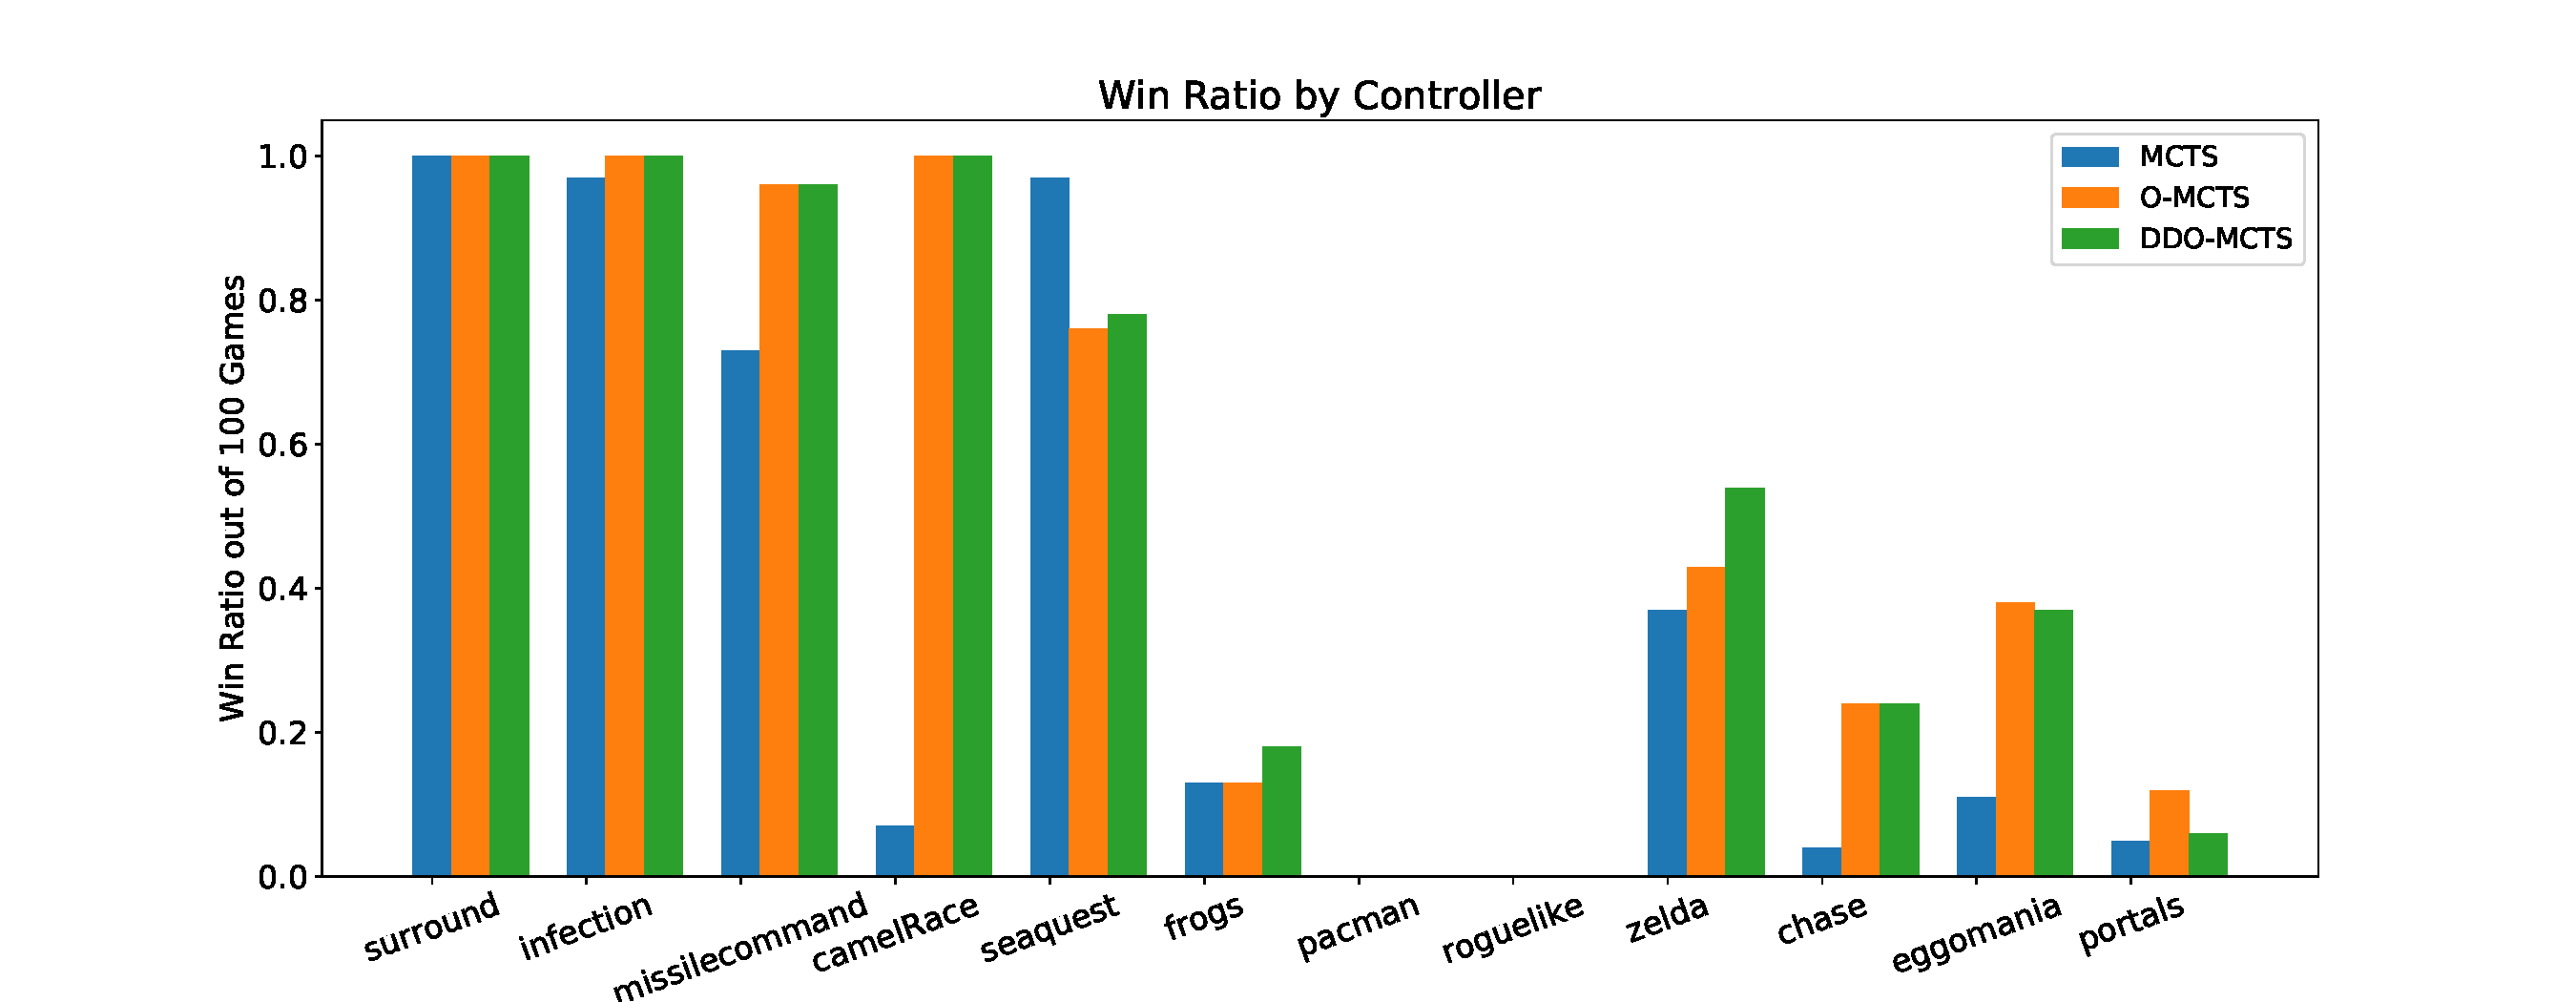
\includegraphics[width=\linewidth]{win_ratio_main.pdf}
    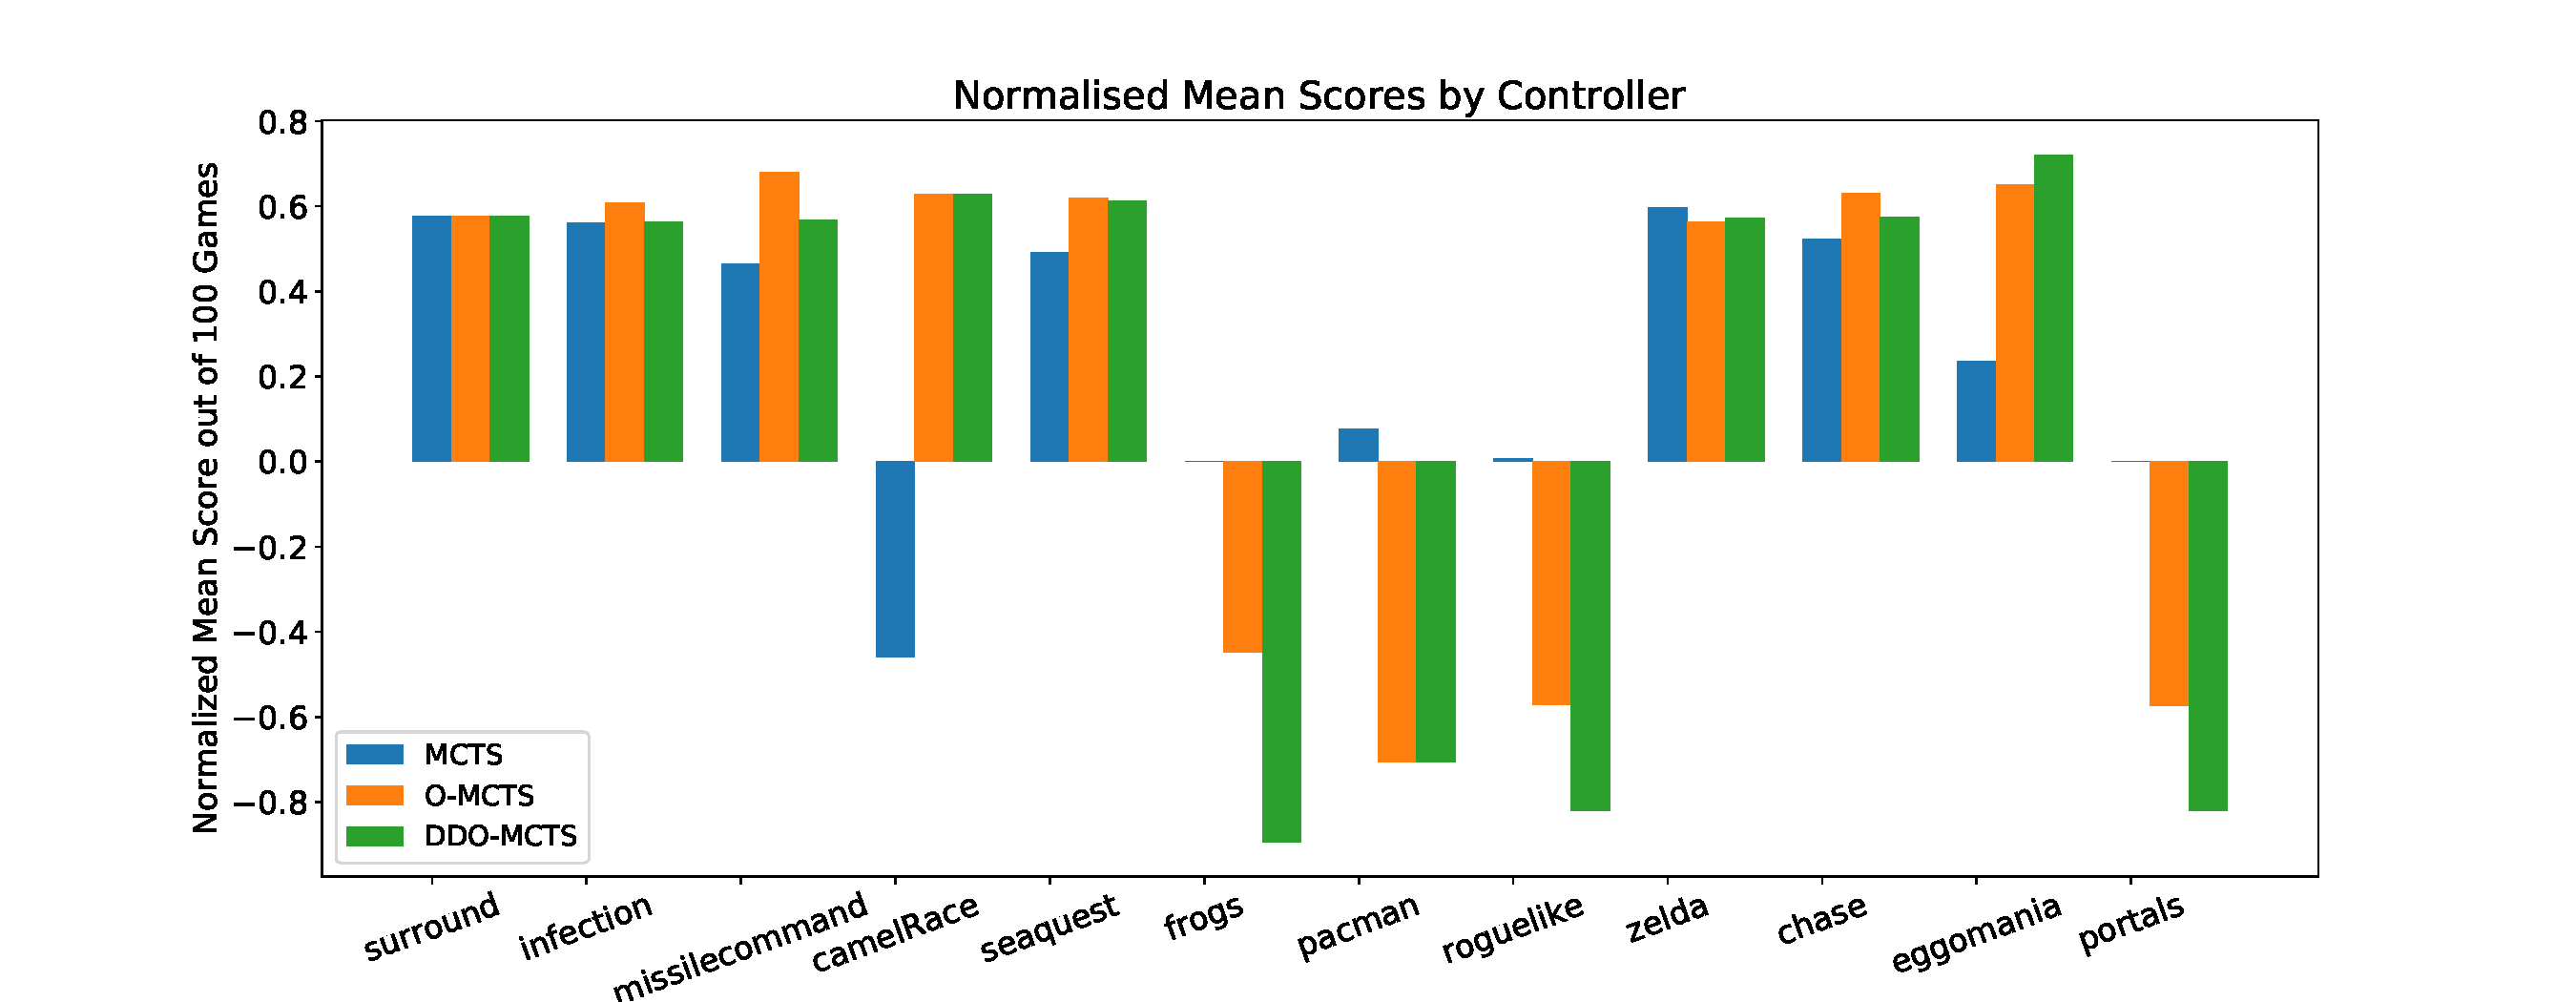
\includegraphics[width=\linewidth]{mean_scores_main.pdf}
    \caption{Win Ratio and Normalised Mean Scores Compared between MCTS, O-MCTS and DDO-MCTS, on a set of 12 games from GVG-AI. Each game is run 100 times.}
    \label{fig:thesis-res}
\end{figure*}

\section{Extension: Hyperparameter Optimisation}
\subsection{Intro}
DDO-MCTS's performance is only benchmarked using a non-unique set of discount factors for each option. However, per-decision option discounting also allows for each option's discount factor, $\gamma_{d}$, to be set individually. In this the following subsections, we explore a method of tuning each option's discount factor $\gamma_{d}$ to be set individually, based on sampled simulations run against the same set of games as before.

\subsection{Motivation}
Some options take longer than others to complete, and using the same $\gamma_{d} = 0.95$, as done in section 5, does not coincide with the motivation of per-decision option discounting, where an agent is supposed to acquire a sense of payoff for a longer strategy, in order to get a larger reward.

\subsection{$\gamma_{d}$ tuning}
In order to tune the discount factor $\gamma_{d}$, the average number of steps for each option duration is used in order to get a ranking among the options. It is sensible to give options with a larger average step count a larger discount factor $\gamma_{d}$ as well.

In this section, we introduce $\gamma_d$ tuning, a method for tuning the individual decision step discounts for options. This method requires a preset $\gamma_{floor}$, or $\gamma_{f}$ for short, which will act as a lower bound for the decision step discount for all options.

Equation \eqref{eq:gamma-tuning} shows how $\gamma^o_{d}$ can be calculated for some option o, using some preset $\gamma_{f}$. The first two lines are just declarations of the vector $\mathbf{x}$ containing all average step counts for all options o, as well as referencing a single average step count for some option o in the vector $\mathbf{x}$, namely, by $x^o$. In the third line, the total average step count over all options is calculated and stored in $\mu$, for use in line four to calculate the normalised value of $x^o$. This normalised value, $\^{x}^o$, is then used as a sort of stretch in line 5.

For example, say $\gamma_{f} = 0.90\  \gamma_{r}$, and $\^{x}^o = 0.78$, then $\gamma^o_{d} = 0.98$, whereas if $\^{x}^o = 0.38$ for some other option o, then $\gamma^o_{d} = 0.94$. The option with the larger step count will get a larger discount factor. However, no matter how small the average step count for some option is, it will not be lower than $\gamma_{floor}$. In other words, $\gamma_d$ tuning squeezes the the average steps of each option in the range of $\gamma_r \leq \gamma_d < 1$.

\begin{equation}
    \begin{align*}
        \mathbf{x} & = average\ step\ counts\ for\ all\ options \\
        x^o &  = average\ step\ count\ for\ option\ o \\
        \mu & = Mean\big(\mathbf{x}\big) \\
        \^{x^o} & = Norm\big(x^o, \mu\big) \\
        \gamma^o_{d} & = \big(\big(1-\gamma_{f}\big)\^{x^o}\big) + \gamma_{f} \\
    \end{align*}
    \label{eq:gamma-tuning}
\end{equation}

\subsection{Experimental Setup}
To evaluate the effectiveness of DDO-MCTS with $\gamma_{d}$ tuning, we compare DDO-MCTS's performance with two different $\Gamma$ sets, one using $\gamma_{f} = 0.9$ and one using $\gamma_{f} = 0.95$. With $\gamma_f = 0.9$, all the decision step discounts will be larger than the regular reward step discount, as per the requirement of per-decision option discounting, $\gamma_d > \gamma_f = \gamma_r$. However, because $\gamma_d = 0.95$ in the section 5, this is also a sensible floor value for the decision step discount factors.

A subset of the games used in section 5, in which both O-MCTS and DDO-MCTS performed relatively well, are used as a benchmark, in order to see if $\gamma_{d}$ tuning introduces some performance benefits. 

To get the average steps for each option, we ran DDO-MCTS on the set of games for 10 simulations each, but this time it only output how many timesteps an option took when it was finished running. A Python script collected the average step counts for each option, and used $\gamma_{d}$ tuning to get individual decision step discount factors for each option, using both $\gamma_f = 0.9$ and $\gamma_f = 0.9$.

\begin{table}[H]
\scriptsize
\begin{tabular}{|l|l|l|l|}
\hline
\multicolumn{1}{|c|}{\multirow{2}{*}{\textbf{Option}}} & \multicolumn{1}{c|}{\multirow{2}{*}{\textbf{Average Steps (X)}}} & \multicolumn{2}{c|}{\textbf{$\gamma_d$}} \\ \cline{3-4} 
\multicolumn{1}{|c|}{}                                 & \multicolumn{1}{c|}{}                                            & $\gamma_f = 0.9$    & $\gamma_f = 0.95$    \\ \hline
\textbf{Option 1}                & 1.09                                                             & 0.91              & 0.95               \\ \hline
\textbf{Option 2}                            & 5.29                                                             & 0.94              & 0.97               \\ \hline
\textbf{Option 3}                             & 6.93                                                             & 0.95              & 0.97               \\ \hline
\textbf{Option 4}                           & 10.95                                                            & 0.98              & 0.99               \\ \hline
\end{tabular}
\caption{$\gamma_d$ tuning results run on options 1 through 4}
\end{table}

The table above shows the output of $\gamma_d$ tuning for the two $\gamma_f$ values, which are the decision step discount factors used in the experiment. On the set of games run, only four options were chosen frequently. The options are GoToNearestSpriteOfItypeOption, GoToPositionOption, GoToMovableOption, GoNearMovableOption, respectively.

\subsection{Results & Evaluation}
Same as before, figure \ref{fig:extens-res} shows the win ratio for each DDO-MCTS agent with the different $\gamma$ discount factor parameters, as well as the normalised mean scores for these games. In three out of the seven games, namely eggomania, seaquest and frogs, we observe that DDO-MCTS without any kind of $\gamma_d$ tuning outperforms those that do. However, in the other four games, one or both of the $\gamma_d$ tuning methods did show improvement. Missilecommand and portals had increased win ratio as $\gamma_f$ was increased to $.95$. Chase, on the other hand, saw the most benefit from $\gamma_d$ tuning with $\gamma_f = 0.9$.

Looking at the normalised avarage scores in the bottom graph of figure \ref{fig:extens-res}, note how in eggomania, seaquest and frogs, reward is lower when using $gamma_d$ tuning, a conclusion shared by the win/loss ratios for these same games. A dramatic improvement is seen in the game portals, where DDO-MCTS without any $gamma_d$ tuning performs not only worse in terms of win/loss ratio, but accumulates a very high negative average reward, whereas DDO-MCTS with $gamma_d$ tuning accumulates zero reward. This could mean that DDO-MCTS without $gamma_d$ tuning will often times choose a shorter option with a lower expected reward than DDO-MCTS with $\gamma_d$ tuning.

These results suggest that $\gamma_d$ tuning can have improve the performance of DDO-MCTS, but it is likely to be very game specific. The average step counts for each option, $\mathbf{x}$, were collected over the same set of games as the agent was tested on. It is possible that $\gamma_d$ tuning only works well when the average step count is collected for each game as well. Although DDO-MCTS with $\gamma_d$ tuning shows some performance improvement for some parameters in some games, it is hard to justify it to be a reliable method of getting a good performance increase in general video games. 

\begin{figure*}
    \centering
    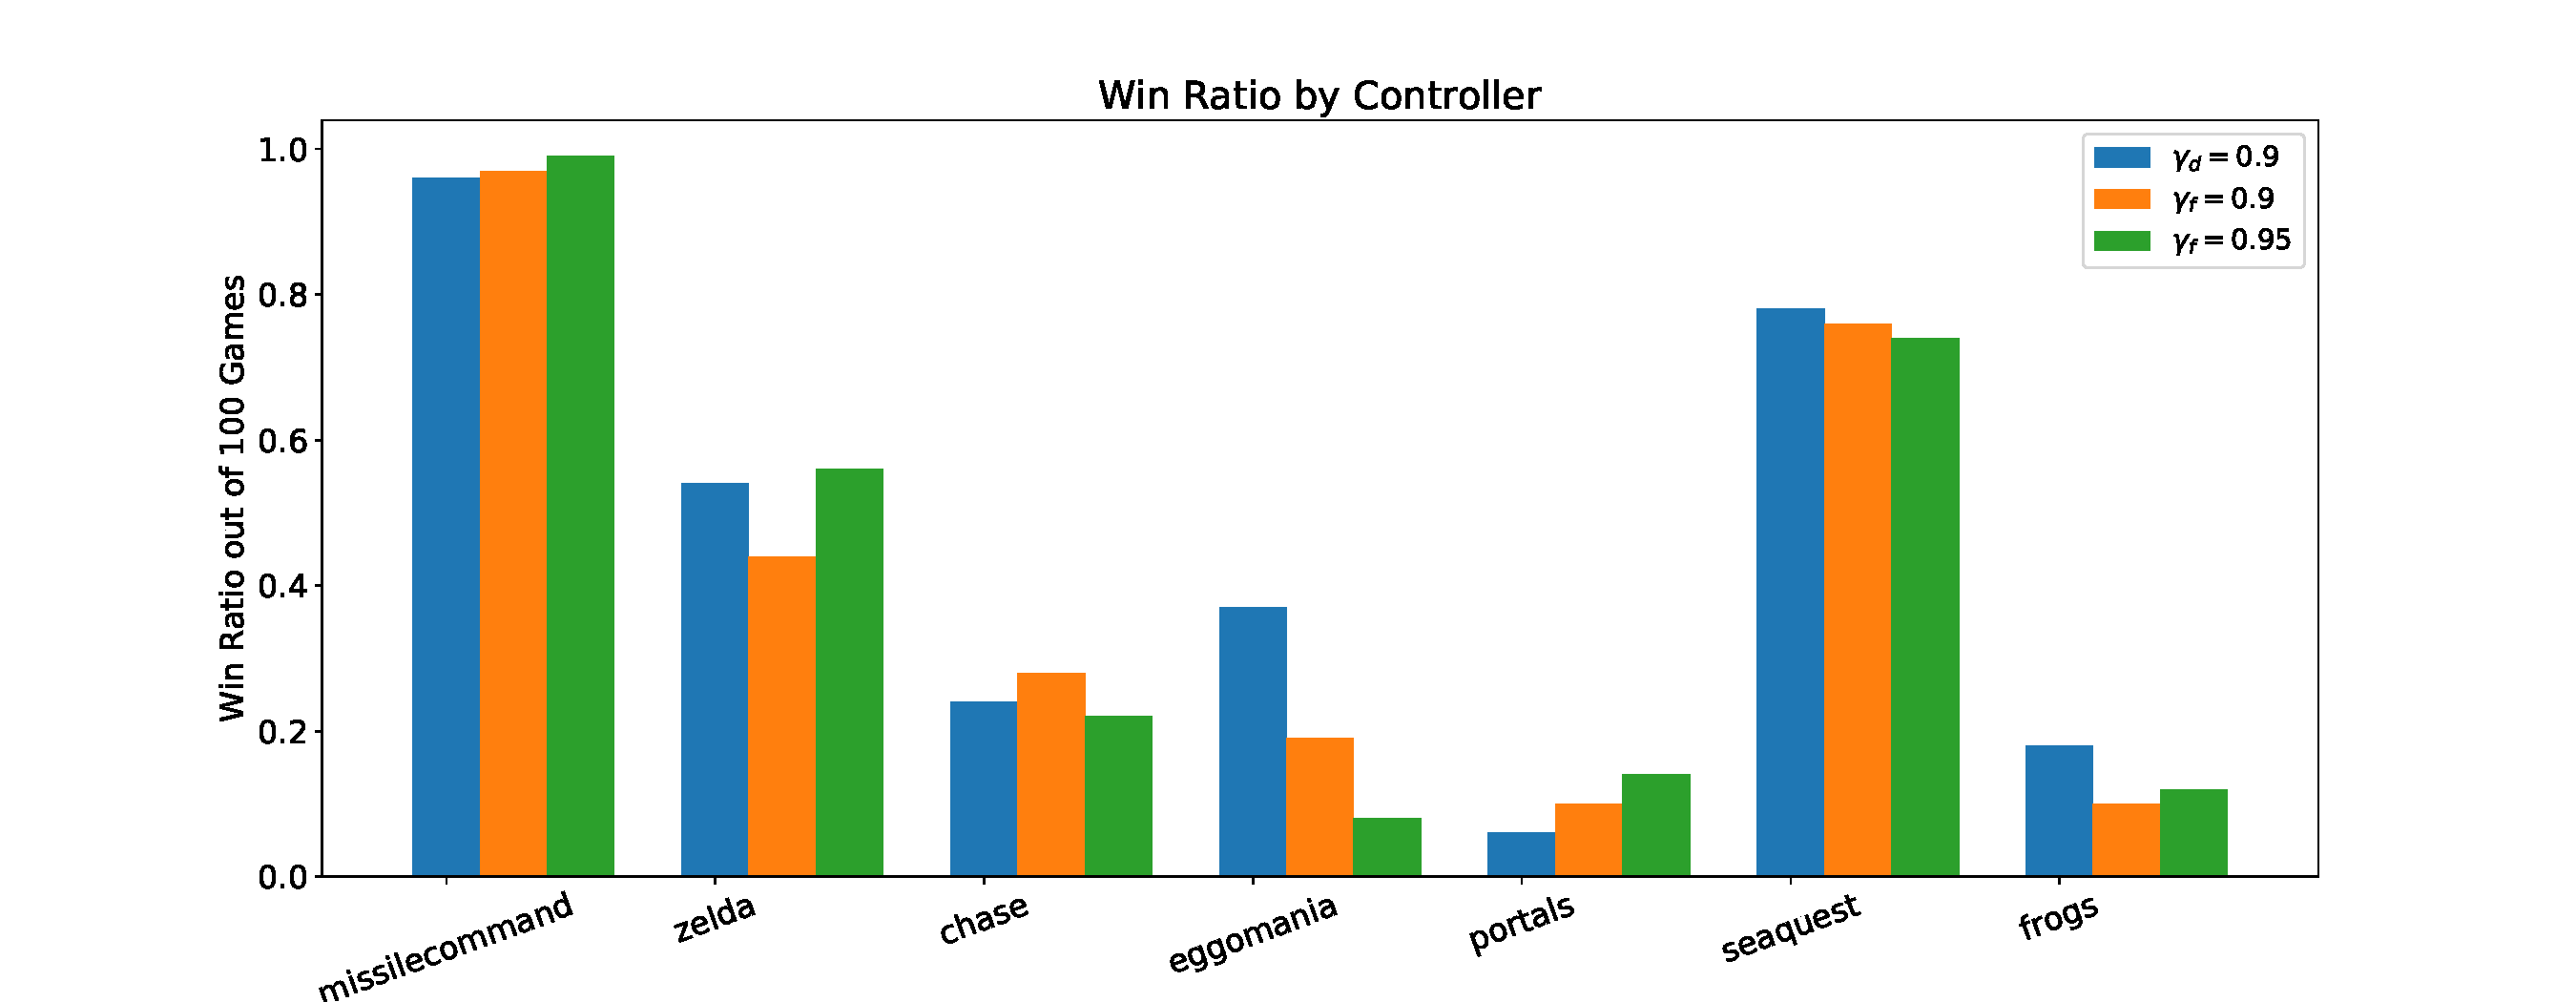
\includegraphics[width=\linewidth]{win_ratio_gamma.pdf}
    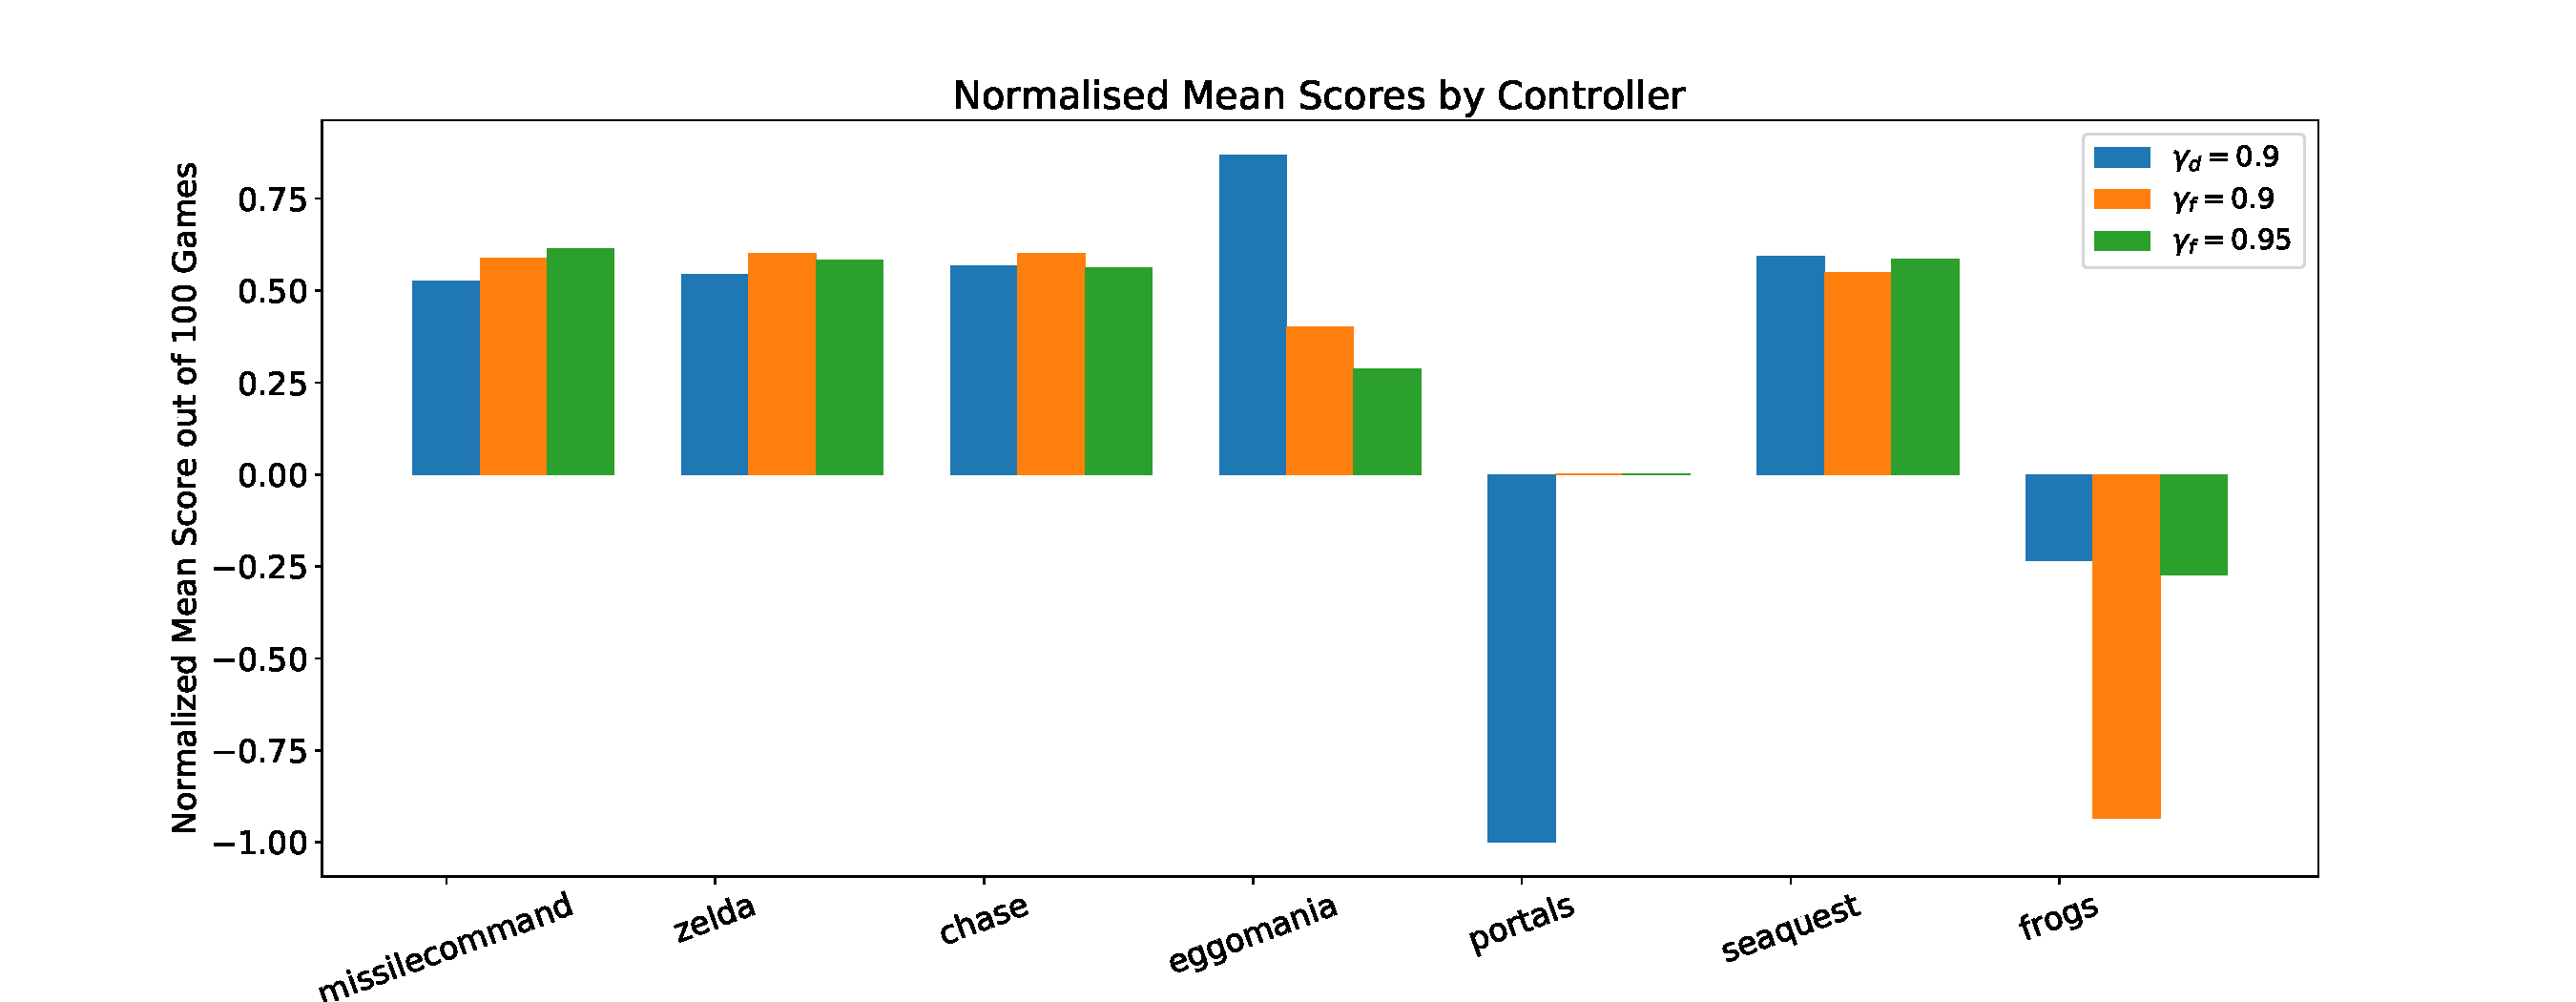
\includegraphics[width=\linewidth]{mean_scores_gamma.pdf}
    \caption{Win Ratio and Normalised Mean Scores compared between DDO-MCTS with different $\gamma_d$ tuning parameters, run on a set of 5 games from GVG-AI. Each game is run for 100 simulations.}
    \label{fig:extens-res}
\end{figure*}

\section{Further Work}
DDO-MCTS shows some interesting performance benefits over regular O-MCTS, however, the tuning process seems to be very difficult.However, it does show good performance increase in some games, which means that $\gamma_d$ tuning can be used when trying to tune DDO-MCTS to perform better on a particular game, rather than focusing on a wide range of games. This is because the average option lengths on which $\gamma_d$ tuning is based, may depend on the game played. Option 1 may perform more steps on average than Option 2 in Game A, but perhaps Option 2 has higher average step count than Option 1 in Game B.  With more options, there is more tuning to be done as well. Future work could investigate a form of online tuning, which could collect the average step counts per option on the fly while a game is being played, updating the average step count and average reward received at the end of each option, and then updating the $\gamma$ discount factors according to some variant of $\gamma_d$ tuning. Then for each new game played, reset the values, assuming nothing about the game/environment and the options' average step counts. If a particular option, say Option 1, takes only very short in some games, but in some others takes a longer sequence of actions, then $\gamma_d$ should be adjusted accordingly for each different game.

Furthermore, another improvement over $\gamma_d$ tuning could take into consideration the reward received after an option was completed, instead of only looking at the average step count. Whether or not an option will pay off does not only depend on the length of an option, but also on if the reward is large enough to justify the longer option. Therefore, it would be interesting to perform $\gamma_d$ tuning where both average step and average reward per option are taken into consideration.

\section{Conclusion}
Although, DDO-MCTS shows some promising results for many games containing subgoals over both MCTS and O-MCTS, the tuning process is the biggest hindrance from it becoming a practical algorithm. Only after $\gamma_d$ tuning, are the benefits of DDO-MCTS apparent, but still limited and game-specific. Since $\gamma_d$ tuning requires additional simulations and statistics, this can also be considered as domain specific knowledge, making it not so much a general video game playing algorithm. Despite the performance gain DDO-MCTS has over its predecessors, it is too insignificant to justify the extra time required to tune the discount factors well enough. Perhaps with an improved, on the fly tuning algorithm, DDO-MCTS may become more of a useful algorithm.

\printbibliography

\end{multicols}

\end{document}
